\documentclass[11pt]{article}
\usepackage[utf8]{inputenc}

\usepackage{geometry}
 \geometry{
     a4paper,
     left=25mm,
     top=25mm,
     right=25mm,
     bottom=30mm
 }

%% for colors
\usepackage{xcolor} % must be loaded erly
%% Define vour custom colors
\definecolor{myblue}{HTML}{648FFF}
\definecolor{mypurple}{HTML}{775EF0}
\definecolor{myred}{HTML}{DD2680}
\definecolor{myorange}{HTML}{FE6100}
\definecolor{myyellow}{HTML}{FFB001}
% Create a new command for the colors
\newcommand{\blue}[1]{\textcolor{myblue}{#1}}
\newcommand{\purple}[1]{\textcolor{mypurple}{#1}}
\newcommand{\red}[1]{\textcolor{myred}{#1}}
\newcommand{\orange}[1]{\textcolor{myorange}{#1}}
\newcommand{\yellow}[1]{\textcolor{myyellow}{#1}}
 
%% for tables
% for dashed and dotted lines
\usepackage{tabularray}
\usepackage{booktabs} % For better hlines in tables
% used to add notes to figures and table with fnote command
\newcommand\fnote[1]{\captionsetup{font=small}\caption*{#1}}
% for tables with cells spanning several rows
\usepackage{multirow}
\usepackage{makecell}

%% for grafics and figures
\usepackage{graphicx}
\usepackage{svg}  % to use .svg
\usepackage{tikz}

%% for flexible list items
\usepackage{enumitem}

%% math 
\usepackage{amsmath}
\usepackage{amsthm}
\usepackage{mathtools} 
\usepackage{verbatim} 

%% format of captions and footnotes
\usepackage[font=small,labelfont=bf]{caption}
% flushing left of footnotes
\usepackage[hang,flushmargin]{footmisc}

%% links and urls
\usepackage[hidelinks]{hyperref}
\hypersetup{
    colorlinks=false,
    linkcolor=black,
    filecolor=magenta,      
    urlcolor=blue,
    citecolor=blue,
}
\urlstyle{same}

%% clever referencing and citing rule
\usepackage{cleveref}
\usepackage[sort, numbers]{natbib}
\usepackage{appendix}

%% new setting for \paragraph
\newcommand{\myparagraph}[1]{\paragraph{#1}\mbox{}\\}

%% format of inline code
\definecolor{codeColor}{gray}{0.85}
\usepackage{tcolorbox}
\newtcbox{\ilc}{on line, boxrule=0pt, boxsep=0pt, bottom = 0pt, left=0pt, right =0pt, top = 0pt, arc = 0pt, colback=white, colframe = white, fontupper={\small \ttfamily}}

%% for code snippets
\usepackage{listings}

\title{Title}

\author{\\ \\
Project Report\\
Operating Systems Lecture Spring Semester 20XX \\ \\ \\ \\
University of Basel \\
Faculty of Science \\
Department of Mathematics and Computer Science \\ \\ \\ \\
FirstName1 LastName1 \\ 
FirstName2 LastName2 \\ \\ \\ \\}
\date{Month DD, 20XX \vfill 
\includegraphics{resources/logo.jpg}}

\begin{document}
    \maketitle
    \thispagestyle{empty}

    \clearpage
    \pagestyle{empty}
    \tableofcontents
    \clearpage    
    \pagestyle{plain}
    \setcounter{page}{1} % Start from page 1
    
    %% Here you add additional files for additional sections
    \section{Introduction}\label{sec:intro}

Use \verb|\cite{}| to cite or reference online sources as in \cite{h5py}, articles like \cite{Dalcin2021}, or articles in proceedings \cite{Alsaadi2021} as defined in references.bib.

\subsection{Subsection Figures} %% t=top, b=bottom, h=here
\begin{figure}[h]
    \centering
    
\includegraphics[width=1.0\linewidth]{figures/terminal.png}
    \caption{Caption for Figure below the Figure}
    \label{fig:example}            
\end{figure}

\subsection{Subsection Tables}
Fancy table:

\begin{table*}[h] %% t=top, b=bottom, h=here
    \centering
    \caption{Caption of Tables above the Table}
    \label{tab:tab}
    \begin{tblr}{width=1\textwidth, colspec={Q[l,m,wd=30mm]|Q[c,m,wd=50mm]|Q[r,m,wd=50mm]},stretch=1.2} 
        Col1 & Col2 & Col3 \\ 
        \hline\hline
% Applications -----------------------------                      
        \SetCell[r=2]{m} 2 row entry & 
        \SetCell[r=1]{m} \makecell[c]{\blue{1 row entry in color}} &
        \makecell[r]{Multirow: 10, 20, 50, 100\\
        1, 2, 4, 8}  \\  
        \cline[dashed]{2-3}
         & \SetCell[r=1]{m} \makecell[c]{\red{1 row entry another color}} &
        \makecell[r]{Multirow:  10'000\\
        2, 4, 8} \\     
        \hline    
% -----------------------------         
        Single Row Left & Center & 
        Right \\  
        \hline\hline
    \end{tblr}
\end{table*} 

    %% References, add them to references.bib
    \bibliographystyle{ieeetr}
    \bibliography{references}
    \addcontentsline{toc}{section}{References}

    \clearpage
    \appendix
     % Redefine the section command for appendices to include the appendix label and number in the title
    \let\oldsection\section
    \renewcommand{\section}[1]{
      % Increment the chapter counter right away
      \refstepcounter{section}
      % Manually format the chapter title to include the appendix label on a separate line and potentially in a smaller font
      % Adjust this line to match your template's specific styling needs
      \oldsection*{{\appendixname\ \thesection}: #1}
      % Add the custom TOC entry with the correctly incremented chapter number
      \addcontentsline{toc}{section}{\appendixname\ \thesection: #1}
    }
    \section{Plots}\label{sec:appendixA}



\section{Materials}\label{sec:appendixB}
\subsection{Software Requirements}\label{SwReq}
Requrements we set ourselves at the initial project submission:
\begin{itemize}
    \item custom data structure
    \item possibility to open files
    \item utf8 support
    \item line break styles
    \item move cursor
    \item clickable buttons
    \item selectable text
    \item edit text
    \item special functions: find, replace
    \item copy ,paste
    \item handle different line break standards
    \item word count statistic
    \item line break type statistic
\end{itemize}
Additional requirements we managed to do:
\begin{itemize}
    \item cursor position statistic
    \item line statistic 
    \item replace all occurences
\end{itemize}
    \clearpage
\section{Declaration of Independent Authorship}\label{sec:integrity}

Copy text from \url{https://dmi.unibas.ch/fileadmin/user_upload/dmi/Studium/Computer_Science/Diverses/Verwendung_AI/2025-02-17_Eigenstaendigkeitserklaerung_Declaration-of-Independent-Authorship_DE_EN_neu.pdf}


\noindent\Large{\textbf{And sign it (all authors!)}}

\begin{figure}[b]
    \centering
    % trim = <left> <bottom> <right> <top>
    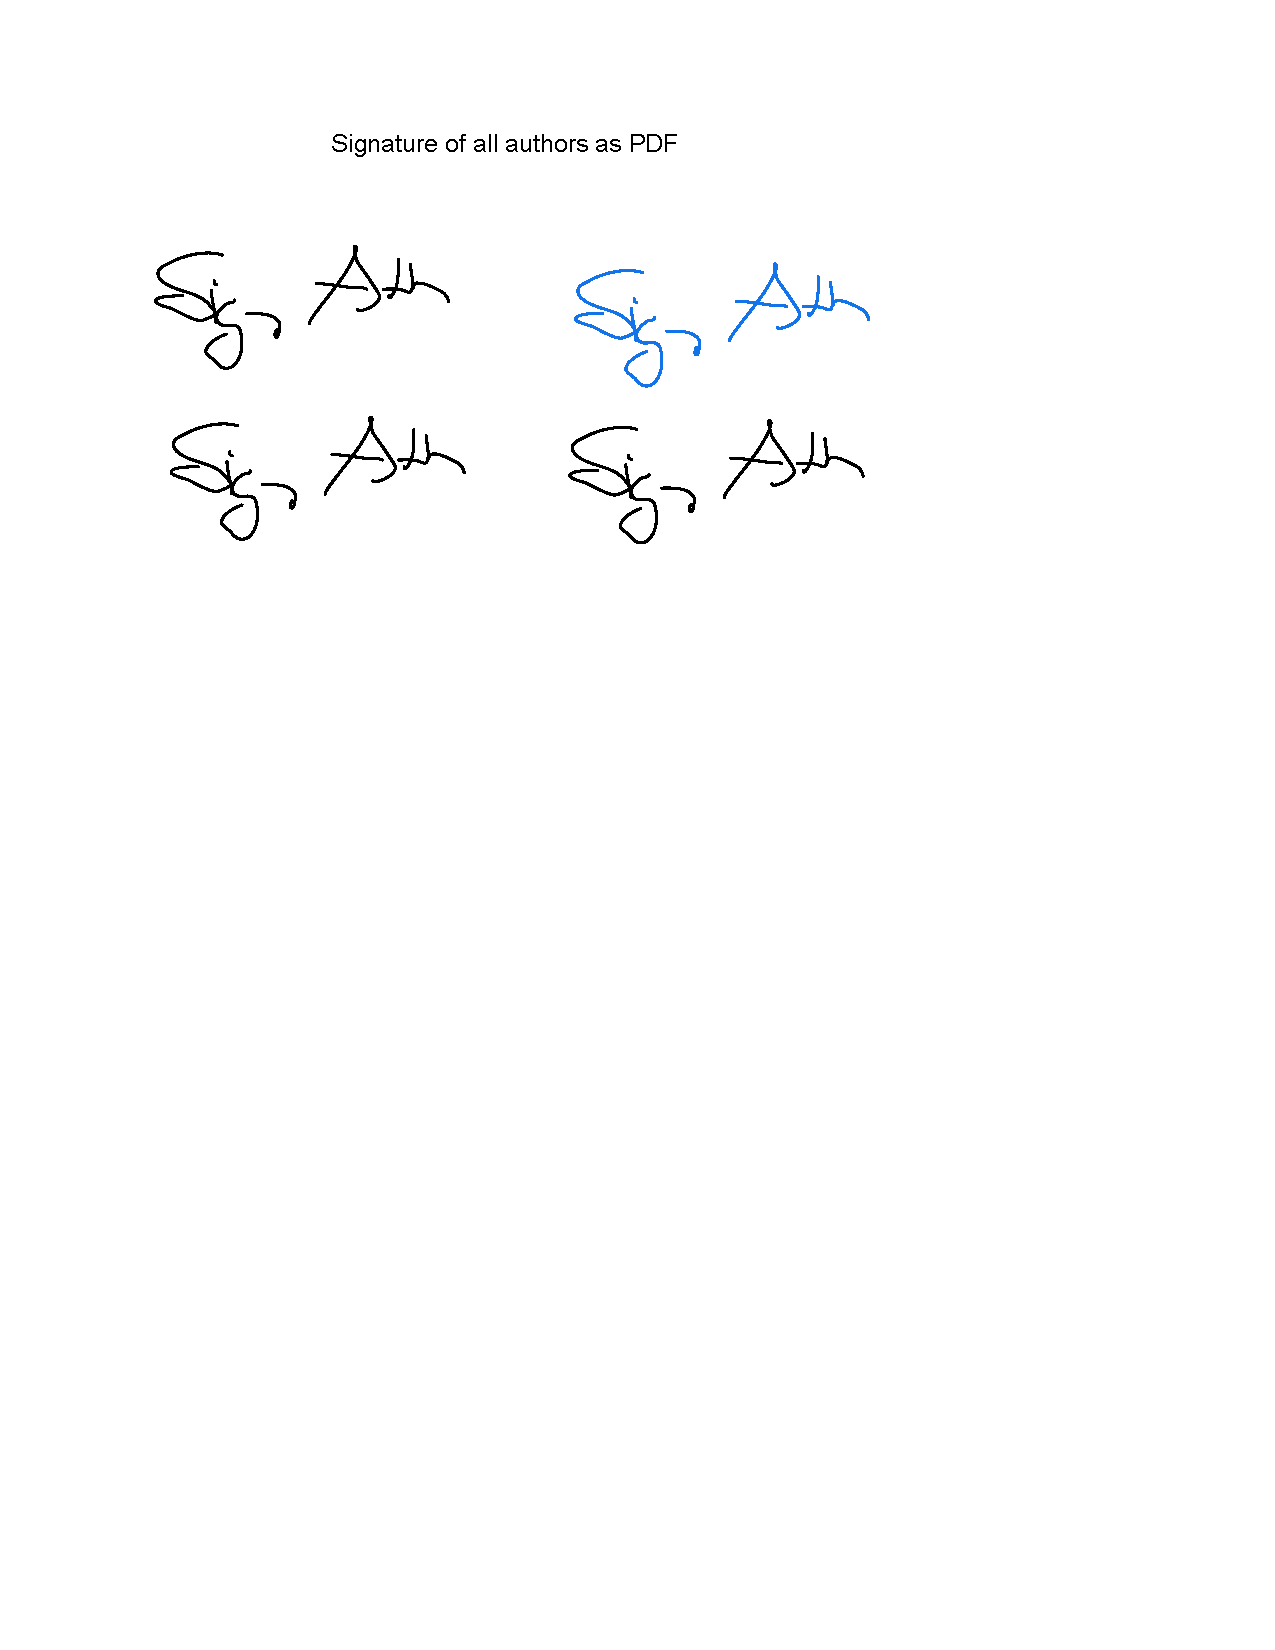
\includegraphics[width=1\textwidth, trim=0pt 500pt 0pt 50pt, clip]{images/example.pdf}
\end{figure}



\end{document}
